\documentclass{beamer}


\usepackage[utf8]{inputenc}
\usepackage{amsmath}
\usepackage{amsfonts}
\usepackage{amssymb}
\usepackage{graphicx}
\usepackage{ragged2e}  % `\justifying` text
\usepackage{booktabs}  % Tables
\usepackage{tabularx}
\usepackage{tikz}      % Diagrams
\usetikzlibrary{calc, shapes, backgrounds}
\usepackage{amsmath}
\usepackage{amssymb}
\usepackage{dsfont}
\usepackage{url}       % `\url
\usepackage{listings}  % Code listings
\usepackage[T1]{fontenc}
\usepackage[percent]{overpic}
\usetikzlibrary{trees}
\usepackage[absolute,overlay]{textpos}
\usepackage{tcolorbox}
\usepackage{menukeys}


\newtcolorbox{terminal}{colback=black!70!white,colframe=black!70!white}
\newtcolorbox{focus}{colback=black!10!white,colframe=black!10!white}
\newtcolorbox{terminal2}[1]{colback=white,colframe=black!70!white,fonttitle=\bfseries,title=#1}

\usepackage{theme/beamerthemehbrs}
\usepackage[normalem]{ulem}
\author[MAS]{Hassan Umari}
\title{ROS Actions}
\subtitle{Foundation Course}
\institute[HBRS]{Hochschule Bonn-Rhein-Sieg}
\date{\today}
\subject{ROS workshop}

% \thirdpartylogo{path/to/your/image}


\begin{document}
{
\begin{frame}
\titlepage
\end{frame}
}


\section{Recap}
\begin{frame}{Recap}
    \framesubtitle{Summary of yesterday’s session}
    We saw that ROS services allow for \textbf{two-way communication} between nodes. However:
    \vspace{5mm}
    \begin{enumerate}
        
        \item Client \textbf{must wait} for the response: a call to a service blocks the code until the execution of the service is finished.
        \vspace{2mm}
        \item During execution of the service, the client cannot ask the server to cancel the request; \textbf{services are not preemptable}.

        \vspace{2mm}
        \item During execution of the service, there is \textbf{no} way for the server to send \textbf{feedback} to the client.


    \end{enumerate}
\end{frame}


\begin{frame}{Recap}
    \framesubtitle{Summary of yesterday’s session}
    

    \begin{enumerate}
        
        \item \textbf{ROS actions} are there to solve these limitations.
        
        \item They are suitable for long-running tasks, which can be interrupted (canceled).
        
        \item Popular case example: sending a pose to the robot, where the action server is responsible for controlling the robot to reach the goal pose.
        
        
    \end{enumerate}
\end{frame}



\begin{frame}{Recap}
    \framesubtitle{ROS Concepts}
    
    Concepts related to ROS computation graph:
    
    \begin{enumerate}
        \item \sout{Nodes.}  \checkmark
        \item \sout{Topics.} \checkmark
        \item \sout{Messages.} \checkmark
        \item \sout{Master.} \checkmark
        \item \sout{Services}. \checkmark
        \item Actions
        \item \sout{Parameter Server.} \checkmark
        \item Bags.
    \end{enumerate}
\end{frame}

\section{ROS Actions}

\begin{frame}{ROS Actions}

    {\huge Actions:}
    \vspace{0.2cm}
    \begin{itemize}
        \item Communication happens between two nodes, the action \textbf{server} node, and the action \textbf{client} node.
        
        \vspace{2mm}
        
        \item A client node sends a \textbf{goal} to the action server. The client does NOT have to wait for the response.
        
        \vspace{2mm}
        
        \item The server node executes the action, during execution it can optionally send feedback messages to the client.
        
    \end{itemize}  
\end{frame}


\begin{frame}{ROS Actions}
    
    {\huge Actions:}
    \vspace{0.2cm}
    \begin{itemize}

        
        \item Meanwhile, the client can receive \textbf{feedback} messages from the server, it can also check on the \textbf{status} of the current goal, or can even ask the server to \textbf{cancel} the action.
        
        \vspace{2mm}
        
        \item Once the server has finished executing the action, it sends a \textbf{result} message back to the client.
    \end{itemize}  
\end{frame}


\begin{frame}{ROS Actions}
 \centering
 \includegraphics[width =0.75\linewidth]{figures/actions.eps}
  
  \vspace{5mm}
 \tiny{\textit{extracted and edited from:       
   \href{http://wiki.ros.org/actionlib/DetailedDescription}{http://wiki.ros.org/actionlib/DetailedDescription}  }}                                                         
\end{frame} 



\begin{frame}{ROS Actions}
    
    {\huge Actions:}
    \vspace{0.2cm}
    \begin{itemize}
        
        
        \item ROS actions are built on top of ROS messages, they are not part of {\ttfamily \colorbox{gray!30!white}{\href{https://docs.ros.org/kinetic/api/rospy/html/}{rospy}}}. 
        
        \vspace{3mm}
        
        \item They are provided in the {\ttfamily \colorbox{gray!30!white}{actionlib}} ROS stack which is installed by default when you install ROS.
       
    \end{itemize}  
\end{frame}


\begin{frame}{ROS Actions}
    
    {\huge Actions:}
    \vspace{0.2cm}
    \begin{itemize}
               
        \item There are no command-line tools to introspect ROS actions.
        
        \begin{itemize}
            \item Example: there is no {\ttfamily \colorbox{gray!30!white}{rosaction list}} command!
            \item Since {\ttfamily \colorbox{gray!30!white}{actionlib}} is built on top of ROS messages, an action server exposes the following topics which can be used for introspection:
            
            \begin{itemize}
                \item {\ttfamily /<action name>/cancel}
                \item {\ttfamily /<action name>/feedback}
                \item {\ttfamily /<action name>/goal}
                \item {\ttfamily /<action name>/result}
                \item {\ttfamily /<action name>/status}
            \end{itemize}
            
        \end{itemize}
        
        
    \end{itemize}  
\end{frame}


\subsection{Action Description Files}

\begin{frame}{Action Description Files}
    \framesubtitle{.action file format}
    \begin{itemize}
        \item A ROS action is defined in a text file with  {\ttfamily \colorbox{yellow}{.action}} extension.
        \item {\ttfamily \colorbox{yellow}{.action}} files are normally placed (not a must) in {\ttfamily \colorbox{gray!30!white}{action}} folder inside the package.
    \end{itemize}
    \vspace{2mm}
    \includegraphics[width=1\linewidth]{figures/package.png}
\end{frame}


\begin{frame}{Action Description files}
    \framesubtitle{.action file format}
    \begin{itemize}
        \item The file consists of three sections: \textbf{goal} message, \textbf{feedback} message, and \textbf{result} message, each separated with "\ttfamily{\textemdash\textemdash\textemdash}":
        
        \vspace{3mm}
        
        \begin{focus}
            \ttfamily{
                fieldtype  \hspace{0.5cm} fieldname\\
                fieldtype  \hspace{0.5cm} fieldname\\
                \textemdash \textemdash \textemdash \\
                fieldtype  \hspace{0.5cm} fieldname\\
                fieldtype  \hspace{0.5cm} fieldname\\
                \textemdash \textemdash \textemdash \\
                fieldtype  \hspace{0.5cm} fieldname\\
                fieldtype  \hspace{0.5cm} fieldname}            
        \end{focus}
    \end{itemize}     
\end{frame}

\begin{frame}{Action Description files}
    \framesubtitle{.action file format}
    \begin{itemize}
        \item Example {\ttfamily \colorbox{yellow}{.action}} file:
        \begin{focus}
            \ttfamily
            geometry\_msgs/PoseStamped  \hspace{0.5cm} target\_pose\\
            \textemdash \textemdash \textemdash \\
            \textemdash \textemdash \textemdash \\
            geometry\_msgs/PoseStamped  \hspace{0.5cm} base\_position\\
        \end{focus} 
    \end{itemize}      
\end{frame}


\begin{frame}{Action Description files}
    \framesubtitle{.action file format}
    
    \begin{itemize}
    \item When you build your package, Catkin reads {\ttfamily \colorbox{yellow}{.action}} file and generates the following ROS messages {\scriptsize (below files are generated from {\ttfamily \colorbox{yellow}{DoDishes.action}} file)}:
    
    \vspace{2mm}
    
    \begin{itemize}
            \item {\ttfamily DoDishesAction.msg}.
            \item {\ttfamily DoDishesActionGoal.msg}.
            \item {\ttfamily DoDishesActionResult.msg}.
            \item {\ttfamily DoDishesActionFeedback.msg}.
            \item {\ttfamily DoDishesGoal.msg}.
            \item {\ttfamily DoDishesResult.msg}.
            \item {\ttfamily DoDishesFeedback.msg}.
    \end{itemize}
    
    \vspace{2mm}
    \item Let's see how to build a package with action files in the next exercise.
    
    \end{itemize}      
\end{frame}


\setbeamercolor{background canvas}{bg=yellow}
\begin{frame}[plain]{}  
    \centering
    {\huge \textcolor{black}{Exercise 1}}
\end{frame}
\setbeamercolor{background canvas}{bg=white}



\subsection{{\ttfamily actionlib} overview}


\begin{frame}{{\ttfamily actionlib} overview}
    The {\ttfamily actionlib} stack provides two Python classes (also in C++) which you can use to implement an action server:
    \vspace{5mm}
    \begin{itemize}
        \item {\ttfamily \color{red} ActionServer} class:
        
         this allows you to define action servers that can accept multiple goals concurrently. {\scriptsize (spanning multiple threads)}
        

    \end{itemize}      
\end{frame}

\begin{frame}{{\ttfamily actionlib} overview}
 and..
    \begin{itemize}

        \item {\ttfamily \color{red} SimpleActionServer} class:  
        
        this class allows you to define action servers that can only handle one goal at a time. 
        
        \vspace{5mm}
        Quote from {\ttfamily actionlib} documentation:
        
        ``\textit{\scriptsize The SimpleActionServer implements a singe goal policy on top of the ActionServer class.}''
    \end{itemize}      
\end{frame}

\begin{frame}{{\ttfamily actionlib} overview}

    \begin{itemize}
        
        \item Throughout this session, we will only use the {\ttfamily \color{red} SimpleActionServer} class to implement action servers.
        
        \vspace{5mm}
        
        \item For action clients, we will use the {\ttfamily {\color{red} SimpleActionClient}} class.

        
    \end{itemize}      
\end{frame}


\subsection{SimpleActionServer in Python}


\begin{frame}[fragile]{SimpleActionServer in Python}
    \framesubtitle{   ../scripts/00\_simple\_server.py}
    \lstset{language=python,
        basicstyle=\ttfamily\scriptsize,
        keywordstyle=\color{blue}\ttfamily,
        stringstyle=\color{red}\ttfamily,
        commentstyle=\color{green}\ttfamily,
        morecomment=[l][\color{magenta}]{\#},
        showstringspaces=false
    }
    \begin{lstlisting}
#!/usr/bin/env python

import rospy
from actionlib import SimpleActionServer
from my_third_package.msg import MoveTurtleAction

def action_cb(goal):
    print("moving turtle to pose: ", goal)
    # Write here the logic to control turtle
    print("done")
    server.set_succeeded()

if __name__ == "__main__":
    rospy.init_node("move_turtle")
    server = SimpleActionServer("move_turtle_action", 
                                MoveTurtleAction,
                                execute_cb=action_cb)
    
    \end{lstlisting}
\end{frame}



\setbeamercolor{background canvas}{bg=yellow}
\begin{frame}[plain]{}  
    \centering
    {\huge \textcolor{black}{Exercise 2}}
\end{frame}
\setbeamercolor{background canvas}{bg=white}


\begin{frame}{SimpleActionServer in Python}
   
    \begin{itemize} 
         
        \item In the previous script, the action server does not allow goal cancellation.
        
        \vspace{5mm}
        
        \item It does not send any feedback as well.
        
        \vspace{5mm}
        
        \item So it is up to you, the implementer, to make the action server send feedback, make it preemtable, etc..
        
    \end{itemize}      
\end{frame}


\begin{frame}{SimpleActionServer in Python}
    
    \begin{itemize} 
        
        \item Let's now see what might be a better implementation for an action server..
        \vspace{7mm}
        \item Check script {\colorbox{yellow}{\ttfamily 01\_simple\_server.py}}
    \end{itemize}      
\end{frame}



\setbeamercolor{background canvas}{bg=yellow}
\begin{frame}[plain]{}  
    \centering
    {\huge \textcolor{black}{Exercise 3}}
\end{frame}
\setbeamercolor{background canvas}{bg=white}


\subsection{SimpleActionClient  in Python}

\begin{frame}{SimpleActionClient in Python}
    
    \begin{itemize} 
        
        \item Simple \textbf{SimpleActionClient}:
        \vspace{7mm}
        
        Let's check script {\colorbox{yellow}{\ttfamily 02\_simple\_client.py}}
    \end{itemize}      
\end{frame}


\setbeamercolor{background canvas}{bg=yellow}
\begin{frame}[plain]{}  
    \centering
    {\huge \textcolor{black}{Exercise 4}}
\end{frame}
\setbeamercolor{background canvas}{bg=white}

\section{References}
\begin{frame}{References}

    \begin{enumerate}
        \item actionlib full documentation.

        \url{https://docs.ros.org/api/actionlib/html/}
        
        \item \href{http://wiki.ros.org/actionlib}{ROS Wiki {\scriptsize/ actionlib}}. 
        
        \item \href{https://github.com/mas-group/minimal_ros_packages/tree/master/srv_minimal}{MAS {\ttfamily \colorbox{gray!30!white}{minimal\_ros\_packages}} GitHub repository}. {\tiny(build instructions, exact copy) }       

    \end{enumerate}
\end{frame}



\setbeamercolor{background canvas}{bg=black}
\begin{frame}[plain]{}  
    \centering
    {\huge \textcolor{white}{Thank you}}
    
    \vspace{0.5cm}
    
    {\huge \textcolor{white}{Any questions?}}
\end{frame}
\setbeamercolor{background canvas}{bg=white}


\end{document}
